
\subsection{package edu.kit.pse.fridget.client.service}
\begin{figure}[H]
	       \centering
	       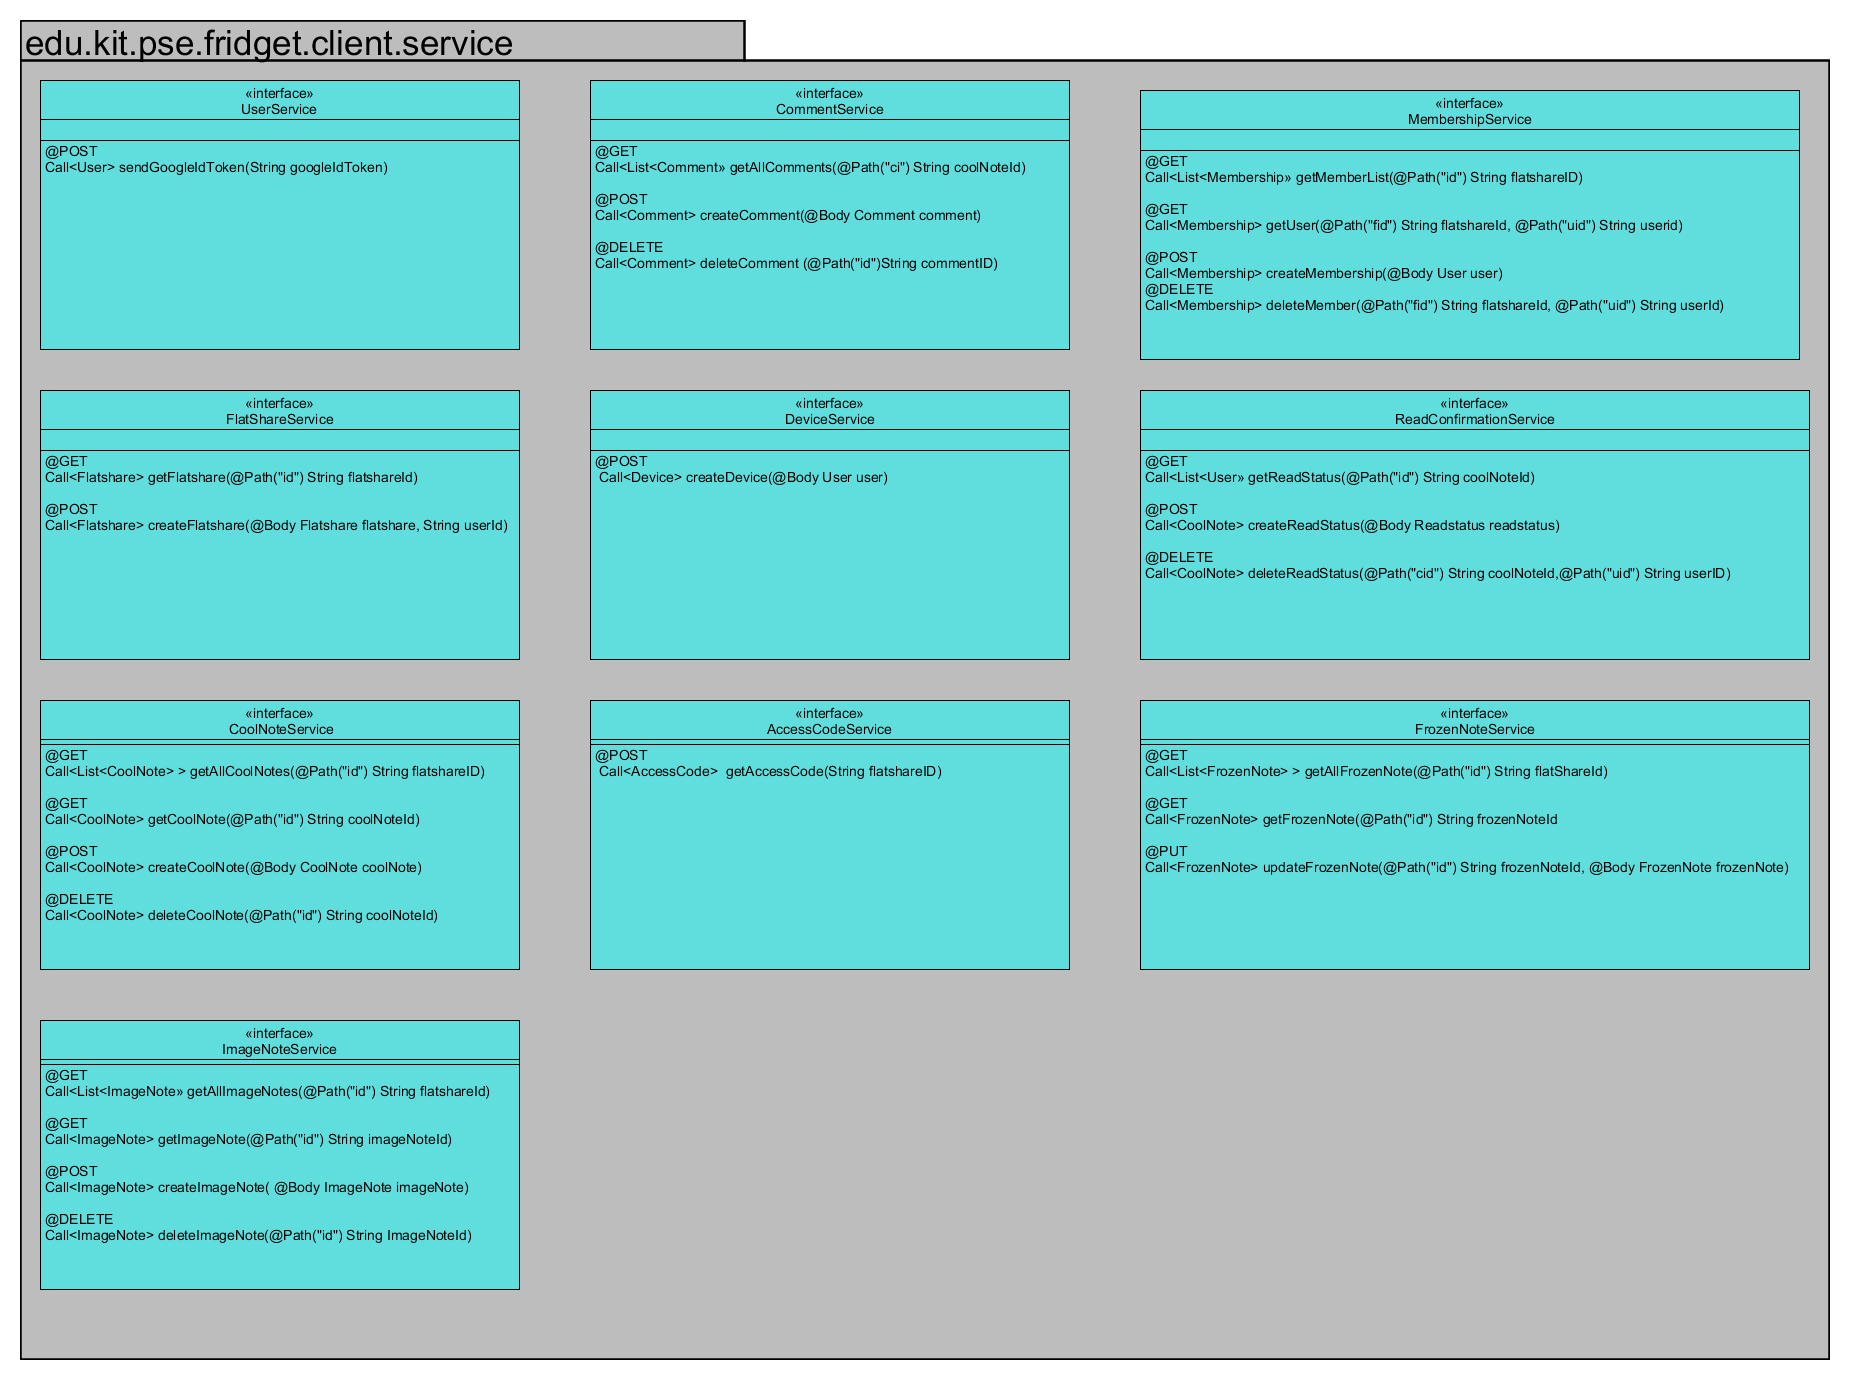
\includegraphics[scale = .26]{service.png}
	       \caption{Klassen des Services}
	      \end{figure}	
	\subsubsection{\texttt{public interface UserService}}
\textit{Dieses Interface dient dazu, den Google-Token an den Server weiterzuleiten.}\\

	\textbf{Methoden}
		\begin{itemize}

      \item\texttt{{@POST\\ Call<User> sendGoogleIdToken(String googleIdToken)}}

		\textit{Diese Methode sendet den GoogleIdToken an den Server}

		\textbf{Parameter}
		\begin{itemize}
			\item\texttt{googleIdToken}
			\textit{zu sendender GoogleToken}
		\end{itemize}
	
		\textbf{Rückgabewert}
		\begin{itemize}
			\item\textit{GoogleToken}
		\end{itemize}		
	

	 \end{itemize}

	\subsubsection{\texttt{public interface AccessCodeService}}
\textit{Dieses Interface ist für die Synchronisation des Accesscodes mit dem Server zuständig }\\
\\
	\textbf{Methoden}
		\begin{itemize}
		\item\texttt{{Call<AccessCode> getAccessCode(String flatShareID)}}

		\textit{Diese Methode fordert den Accesscode einer Flatshare an}

		\textbf{Parameter}
		\begin{itemize}
			\item\texttt{flatshareId}
			\textit {übergebende ID der Flatshare}
		 \end{itemize}
		 
		\textbf{Rückgabewert} 
		\begin{itemize}
		\item\textit{Accesscode der Flatshare}
		\end{itemize}

	 \end{itemize}

		\subsubsection{\texttt{public interface CommentService }}
\textit{Dieses Interface ist für die Synchronisation der Comments mit dem Server zuständig}\\
\\
	\textbf{Methoden} 
		\begin{itemize}
		\item\texttt{{@GET("comments?cool-note=\{cid\}")\\ Call<List<Comment>> getAllComments(@Path(\grqq cid\grqq)String coolNoteId)}}

		\textit{Diese Methode ruft alle Kommentare einer Cool Note ab}

		\textbf{Parameter} 
		\begin{itemize}
			\item\texttt{coolNoteId}
		 	\textit{die ID der Cool Note}
	 	\end{itemize}

		\textbf{Rückgabewert} 
		\begin{itemize}
			\item\textit{Alle Comments der zur CoolNoteId gehörenden Cool Note}
	 	\end{itemize}


      \item\texttt{{@POST("/comments")
\\ Call<Comment> createComment(@Body Comment comment)}}

		\textit{Diese Methode schickt einen Comment an den Server }

		\textbf{Parameter} 
			\begin{itemize}
				\item\texttt{comment}
		 		\textit{speichert einen Comment}
	 		\end{itemize}


		\textbf{Rückgabewert} 
		\begin{itemize}
			\item\textit{Ein Comment}
	 	\end{itemize}
		

	 \item\texttt{{@DELETE("/comments/{id}")\\ Call<Comment> deleteComment (@Path(\grqq id\grqq)String commentID)}}

		\textit{Diese Methode löscht einen Comment }
		
		\textbf{Parameter} 
			\begin{itemize}
				\item\texttt{commentID}
		 		\textit{ID des zu löschenden Comments}
	 		\end{itemize}

	 \end{itemize}


	\subsubsection{\texttt{public interface CoolNoteService }}
\textit{Dieses Interface ist für die Synchronisation der Cool Notes mit dem Server zuständig}\\
\\
	\textbf{Methoden} 
		\begin{itemize}
		\item\texttt{{@GET("/cool-notes?flatshare={id}")\\ Call<List<CoolNote>> getAllCoolNotes(@Path(\grqq id\grqq) String flatshareID)}}

		\textit{Diese Methode ruft alle Cool Notes einer Flatshare ab}

	\textbf{Parameter} 
			\begin{itemize}
				\item\texttt{flatshareId}
		 		\textit{Die Flatshare ID der abzurufenden Cool Notes}
	 		\end{itemize}
	 		
		\textbf{Rückgabewert} 
	\begin{itemize}
			\item\textit{Alle Cool Notes}
	 	\end{itemize}
	

      \item\texttt{{@GET("/cool-notes/{id}")\\ Call<CoolNote> getCoolNote(@Path(\grqq id\grqq) String coolNoteId)}}

		\textit{Diese Methode ruft den Inhalt einer Cool Note ab }
	\textbf{Parameter} 
			\begin{itemize}
				\item\texttt{coolNoteId}
		 		\textit{Die ID der Cool Note}
	 		\end{itemize}

		\textbf{Rückgabewert} 
		\begin{itemize}
			\item\textit{Inhalt der zu der CoolNoteID gehörenden Cool Note}
	 	\end{itemize}	

      \item\texttt{{@POST("/cool-notes")\\ Call<CoolNote> createCoolNote(@Body CoolNote coolNote)}}

		\textit{Diese Methode schickt eine neue Cool Note an den Server }

		\textbf{Parameter} 
			\begin{itemize}
				\item\texttt{coolNote}
		 		\textit{Die Cool Note}
	 		\end{itemize}

		\textbf{Rückgabewert} 
		\begin{itemize}
				\item\texttt{Cool Note}
	 		\end{itemize}

      \item\texttt{{@DELETE("/cool-notes/{id}")\\ Call<CoolNote> deleteCoolNote(@Path(\grqq id\grqq) String coolNoteId)}}

		\textit{Diese Methode löscht eine Cool Note }

	\textbf{Parameter} 
			\begin{itemize}
				\item\texttt{coolNoteId}
		 		\textit{Die Id der Cool Not}
	 		\end{itemize}

	 \end{itemize}


	\subsubsection{\texttt{public interface FlatShareService }}
\textit{Dieses Interface verwaltet die Synchronisation der Flatshare mit dem Server}\\
\\
	\textbf{Methoden} 
		\begin{itemize}
		\item\texttt{{@POST ("/flatshares") \\
Call<Flatshare> createFlatshare(@Body Flatshare flatshare, String userId)
}}

		\textit{Diese Methode erstellt eine neue Flatshare auf dem Server
}
	\textbf{Parameter} 
			\begin{itemize}
				\item\texttt{flatshare}
		 		\textit{Name der zu erstellenden Flatshare}
		 		
		 		\item\texttt{userID}
		 		\textit{ID des Users, der die Flatshare erstellt}
	 		\end{itemize}

		\textbf{Rückgabewert} 
		\begin{itemize}
		\item\textit{Flatshare}
		\end{itemize}

      \item\texttt{{@GET("/flatshares/{id}")\\ Call<Flatshare> getFlatshare(@Path(\grqq id\grqq) 					String flatshareId)}}

		\textit{Diese Methode ruft die Flatshare-Daten vom Server ab}

		\textbf{Parameter} 
			\begin{itemize}
				\item\texttt{flatshareId}
		 		\textit{die ID der aufgerufenen Flatshare}
	 		\end{itemize}

		\textbf{Rückgabewert} 
		\begin{itemize}
		\item\textit{Flatshare}
		\end{itemize}

	 \end{itemize}



	\subsubsection{\texttt{public interface FrozenNoteService }}
\textit{Dieses Interface ist für die Synchronisation der Frozen Notes mit dem Server zuständig}\\
\\
	\textbf{Methoden} 
		\begin{itemize}
		\item\texttt{{@GET("/frozen-notes?flatshare={id}")\\
Call<List<FrozenNote>> getAllFrozenNote(@Path(\grqq id\grqq) String flatShareId)}}

		\textit{Diese Methode ruft die Frozen Notes vom Server ab}

		\textbf{Parameter} 
			\begin{itemize}
				\item\texttt{flatshareId}
		 		\textit{die ID der aufgerufenen Flatshare}
	 		\end{itemize}

		\textbf{Rückgabewert} 
		\begin{itemize}
		\item\textit{Frozen Note}
		\end{itemize}
		
		
      \item\texttt{{@GET("/frozen-notes/{id}")\\ Call<FrozenNote> getFrozenNote(@Path(\grqq id\grqq) String frozenNoteId)}}

		\textit{Diese Methode ruft den Inhalt einer Frozen Note ab }
	
		\textbf{Parameter} 
			\begin{itemize}
				\item\texttt{frozenNoteId}
		 		\textit{die ID der aufgerufenen Frozen Note }
	 		\end{itemize}

		\textbf{Rückgabewert} 
		\begin{itemize}
		\item\textit{Frozen Note}
		\end{itemize}

	 \item\texttt{{@PUT("/frozen-notes/{id}")\\ Call<FrozenNote> updateFrozenNote(@Path(\grqq id\grqq) String frozenNoteId, @Body FrozenNote frozenNote)}}

		\textit{Diese Methode speichert Änderungen in einer Frozen Note}

		\textbf{Parameter} 
			\begin{itemize}
				\item\texttt{frozenNoteId}
		 		\textit{die ID der aufgerufenen Frozen Note }
		 		\item\texttt{frozenNote}
		 		\textit{die geänderte Frozen Note}
	 		\end{itemize}

		\textbf{Rückgabewert} 
		\begin{itemize}
		\item\textit{Frozen Note}
		\end{itemize}

	 \end{itemize}


	\subsubsection{\texttt{public interface ImageNoteService }}
\textit{Dieses Interface dient zur Synchronisation der Image-Cool-Notes mit dem Server}\\
\\
	\textbf{Methoden} 
		\begin{itemize}
		\item\texttt{{@GET("/image-notes?flatshare={id}")\\
Call<List<ImageNote>> getAllImageNotes(@Path(\grqq id\grqq) String flatshareId)}}

		\textit{Diese Methode ruft die Image-Cool-Notes vom Server ab}

		\textbf{Parameter} 
			\begin{itemize}
				\item\texttt{flatshareId}
		 		\textit{die ID der aufgerufenen Flatshare}
	 		\end{itemize}

		\textbf{Rückgabewert} 
		\begin{itemize}
		\item\textit{ImageCoolNote}
		\end{itemize}
		
      \item\texttt{{@GET("/image-notes/{id}")\\ Call<ImageNote> getImageNote(@Path("\grqq id\grqq") String imageNoteId)}}

		\textit{Diese Methode ruft eine Image-Cool-Note ab }

		\textbf{Parameter} 
			\begin{itemize}
				\item\texttt{imageNoteId}
		 		\textit{die ID der aufgerufenen Image-Cool-Note}
	 		\end{itemize}

		\textbf{Rückgabewert} 
		\begin{itemize}
		\item\textit{Image-Cool-Note}
		\end{itemize}
		

	\item\texttt{{@POST("/image-notes")\\ Call<ImageNote> createImageNote( @Body ImageNote imageNote)}}

		\textit{Diese Methode schickt ein Image-Cool-Note an den Server}

		\textbf{Parameter} 
			\begin{itemize}
				\item\texttt{imageNote}
		 		\textit{eine Image-Cool-Note}
	 		\end{itemize}

		\textbf{Rückgabewert} 
		\begin{itemize}
		\item\textit{Image-Cool-Note}
		\end{itemize}


	     \item\texttt{{@DELETE("/image-notes/{id}")\\Call<ImageNote> deleteImageNote(@Path("\grqq id\grqq") String ImageNoteId)}}

		\textit{Diese Methode löscht eine Image-Cool-Note}

		\textbf{Parameter} 
			\begin{itemize}
				\item\texttt{imageNoteId}
		 		\textit{Die ID der zu löschenden Image-Cool-Note }
	 		\end{itemize}

	 \end{itemize}


	\subsubsection{\texttt{public interface MembershipService }}
\textit{Dieses Interface verwaltet die Synchronisation der Members mit dem Server}\\
\\
	\textbf{Methoden} 
		\begin{itemize}
		\item\texttt{{@GET("/memberships/users?flatshare={id}") \\ Call<List<Membership>> getMemberList(@Path("id") String flatshareID)}}

		\textit{Diese Methode ruft die Mitglieder einer Flatshare ab}

		\textbf{Parameter} 
			\begin{itemize}
				\item\texttt{flatshareId}
		 		\textit{die ID der aufgerufenen Flatshare}
	 		\end{itemize}

		\textbf{Rückgabewert} 
		\begin{itemize}
		\item\textit{MemberList}
		\end{itemize}


      \item\texttt{{@GET("memberships?flatshare={fid}\&user ={uid}")\\Call<Membership> getUser(@Path("fid") String flatshareId, @Path(\grqq uid\grqq) String userid)}}

		\textit{Diese Methode ruft die Daten eines Members ab}        	

		\textbf{Parameter} 
			\begin{itemize}
				\item\texttt{flatshareId}
		 		\textit{die ID der aufgerufenen Flatshare}
		 		\item\texttt{userId}
		 		\textit{die ID des aufgerufenen Users}
	 		\end{itemize}

		\textbf{Rückgabewert} 
		\begin{itemize}
		\item\textit{Daten eines Members}
		\end{itemize}


      \item\texttt{{@POST("/memberships")\\ Call<Membership> createMembership(@Body User user)}}

		\textit{Diese Methode fügt einen neuen Member in eine Flatshare ein}        	
		
		\textbf{Parameter} 
			\begin{itemize}
				\item\texttt{user}
		 		\textit{ Der User, der zu der Flatshare hinzugefügt wird}
	 		\end{itemize}

	      \item\texttt{{@DELETE("/memberships?flatshare={fid}\&user={uid}")\\Call<Membership> deleteMember(@Path("fid") String flatshareId, @Path("uid") String userId)}}

		\textit{Diese Methode löscht einen Member}        	
		\textbf{Parameter} 
			\begin{itemize}
				\item\texttt{flatshareId}
		 		\textit{die ID der aufgerufenen Flatshare}
		 		\item\texttt{userId}
		 		\textit{die ID des aufgerufenen Users}
	 		\end{itemize}		

	 \end{itemize}

	\subsubsection{\texttt{public interface ReadConfirmationService }}
\textit{Dieses Interface synchronisiert den Gelesen-Status mit dem Server}\\
\\
	\textbf{Methoden} 

    \begin{itemize}
		\item\texttt{{@GET("/read-confirmations/users?cool-note={id}") \\ Call<List<User>> getReadStatus(@Path(\grqq id\grqq) String coolNoteId)}}

		\textit{Diese Methode ruft den Gelesen-Status vom Server ab}

		\textbf{Parameter} 
			\begin{itemize}
				\item\texttt{coolNoteId}
		 		\textit{Die ID der betreffenden Cool Note}
	 		\end{itemize}

		\textbf{Rückgabewert} 
		\begin{itemize}
		\item\textit{Read-Status}
		\end{itemize}

	\item\texttt{{@POST("/read-confirmations") \\ Call<CoolNote> createReadStatus(@Body Readstatus readstatus) }}

		\textit{Diese Methode setzt die Checkbox auf markiert}

		\textbf{Parameter} 
			\begin{itemize}
				\item\texttt{readstatus}
		 		\textit{zeigt den Gelesen-Status einer Cool Note an}
	 		\end{itemize}

		\textbf{Rückgabewert} 
		\begin{itemize}
		\item\textit{ReadStatus}
		\end{itemize}



	\item\texttt{{@DELETE("/read-confirmations?cool-note={cid}\&user={uid}")
\\Call<CoolNote> deleteReadStatus(@Path("cid") String coolNoteId,
			     @Path(\grqq uid\grqq) String userID)}}

		\textit{Diese Methode setzt die Checkbox auf unmarkiert}

		\textbf{Parameter} 
			\begin{itemize}
				\item\texttt{coolNoteID}
		 		\textit{die ID der aufgerufenen Cool Note}
		 		\item\texttt{userID}
		 		\textit{die ID des aufgerufenen Users}
	 		\end{itemize}
	
	 \end{itemize}


	\subsubsection{\texttt{public interface DeviceService }}
\textit{Dieses Interface synchronisiert die Device-Daten mit dem Server}\\
\\
	\textbf{Methoden} \\
		\begin{itemize}
		\item\texttt{{@POST("/devices") \\ Call<Device> createDevice(@Body User user)}}

		\textit{Diese Methode fügt ein Device zu einer Flatshare hinzu}

		\textbf{Parameter} 
			\begin{itemize}
				\item\texttt{user}
		 		\textit{der zu dem Device gehörende User}
	 		\end{itemize}

		\textbf{Rückgabewert} 
		\begin{itemize}
		\item\textit{Device Daten}
		\end{itemize}

	 \end{itemize}